%%%%%%%%%%%%%%%%%%%%%%%%%%%%%%%%%%%%%%%%%
% Stylish Article
% LaTeX Template
% Version 2.0 (13/4/14)
%
% This template has been downloaded from:
% http://www.LaTeXTemplates.com
%
% Original author:
% Mathias Legrand (legrand.mathias@gmail.com)
%
% License:
% CC BY-NC-SA 3.0 (http://creativecommons.org/licenses/by-nc-sa/3.0/)
%
%%%%%%%%%%%%%%%%%%%%%%%%%%%%%%%%%%%%%%%%%

%----------------------------------------------------------------------------------------
%	PACKAGES AND OTHER DOCUMENT CONFIGURATIONS
%----------------------------------------------------------------------------------------

\documentclass[fleqn,10pt,onecolumn]{ipcc} % Document font size and equations flushed left

\usepackage{lipsum} % Required to insert dummy text. To be removed otherwise
\usepackage{tikz} % good quality graphs
\usepackage{pgfplots}
\usepackage[ampersand]{easylist}
\usepackage{listings}
\usepackage{amsmath}
\usepackage{mathtools}
\lstset{language=C} 
\usetikzlibrary{pgfplots.groupplots}
\pgfplotsset{compat=newest}

\lstdefinestyle{customc}{
  belowcaptionskip=1\baselineskip,
  breaklines=true,
  frame=L,
  xleftmargin=\parindent,
  language=C,
  showstringspaces=false,
  basicstyle=\footnotesize\ttfamily,
  keywordstyle=\bfseries\color{green!40!black},
  commentstyle=\itshape\color{purple!40!black},
  identifierstyle=\color{blue},
  stringstyle=\color{orange},
}

\lstset{
  numbers=left,
  stepnumber=1,    
  firstnumber=1,
  numberfirstline=true,
  numberstyle=\color{gray}, % the style that is used for the line-numbers
  rulecolor=\color{black},         % if not set, the frame-color may be changed on line-breaks within not-black text (e.g. comments (green here))
}

%----------------------------------------------------------------------------------------
%	COLUMNS
%----------------------------------------------------------------------------------------

\setlength{\columnsep}{0.45cm} % Distance between the two columns of text
\setlength{\fboxrule}{0.75pt} % Width of the border around the abstract

%----------------------------------------------------------------------------------------
%	COLORS
%----------------------------------------------------------------------------------------

\definecolor{IrishGreen}{RGB}{0,0,90} % Color of the article title and sections
\definecolor{RoyalBlue}{RGB}{0,20,20} % Color of the boxes behind the abstract and headings

%----------------------------------------------------------------------------------------
%	HYPERLINKS
%----------------------------------------------------------------------------------------

\usepackage[colorlinks=true,bookmarks=true,plainpages=false,
linkcolor=IrishGreen, citecolor=IrishGreen, 
urlcolor=IrishGreen,pagebackref]{hyperref}%links in pdf
\usepackage[compress,numbers,comma]{natbib} %references
\usepackage{hypernat} %references
%----------------------------------------------------------------------------------------
%	ARTICLE INFORMATION
%----------------------------------------------------------------------------------------

\JournalInfo{OpenCL Notes} % Journal information
\Archive{} % Additional notes (e.g. copyright, DOI, review/research article)

\PaperTitle{OpenCL Notes} % Article title

\Authors{Christian Lalanne\textsuperscript{1}*, Aditya Chaturvedi\textsuperscript{2}, Rory Gogarty\textsuperscript{2}} % Authors
\affiliation{\textsuperscript{1}\textit{Irish Centre for High End Computing}} % Author affiliation
\affiliation{\textsuperscript{2}\textit{University College Dublin}} % Author affiliation
\affiliation{*\textbf{Corresponding author}: christian.lalanne@ichec.ie} % Corresponding author

\Keywords{OpenCL, GPU, Xeon Phi, Parallelism} % Keywords - if you don't want any simply remove all the text between the curly brackets
\newcommand{\keywordname}{Keywords} % Defines the keywords heading name

%----------------------------------------------------------------------------------------
%	ABSTRACT
%----------------------------------------------------------------------------------------

\Abstract{TBAL}

%----------------------------------------------------------------------------------------
\graphicspath{{figures/}}
%colours
\definecolor{IrishGreen}{cmyk}{0.70, 0.00, 0.80, 0.10}
\definecolor{RoyalBlue}{cmyk}{0.1, 0.0, 0.0, 0.02}

\begin{document}

\flushbottom % Makes all text pages the same height
\maketitle % Print the title and abstract box
\tableofcontents % Print the contents section
\listoffigures % list of figures
\listoflistings %list of listings
\listoftables %list of tables
\thispagestyle{empty} % Removes page numbering from the first page


%----------------------------------------------------------------------------------------
%	ARTICLE CONTENTS
%----------------------------------------------------------------------------------------


\section*{Introduction} % The \section*{} command stops section numbering
\addcontentsline{toc}{section}{Introduction} % Adds this section to the table of contents with negative 
                                            %horizontal space equal to the indent for the numbered sections
\par{Molecular dynamics techniques grew rapidly in the last twenty years. 
The grow was fuelled by development of new scalable mathematical algorithms, availability 
of powerful hardware and better availability of ready to use software packages. DL\_POLY is one of 
these packages, widely adopted by the computational physics and material science communities.}
\par{DL\_POLY started its life in 1994 at Daresbury Laboratory, now part of Science \& Technology Facilities 
Council in United Kingdom. The main developers for the currect version are W Smith and IT Todorov. DL\_POLY is 
a general classical molecular dynamics code and was used to simulate macro molecules (both biological and synthetic),
complex fluids, materials and ionic liquids. DL\_POLY also plays an important role as sandbox for both development
of new methods and algorithms for molecular dynamics and testing of emerging hardware 
technologies\cite{dlpoly} and \cite{Todorov2006}.
The core code is written in Fortran 90 and optimised for distributed systems using domain decomposition, also OpenMP and CUDA ports exist as 
contributions to DL\_POLY but not part of the official distribution.
DL\_POLY is free of use for UK academics pursuing non-commerical research and available for licensing for the rest.
Over 3000 licenses were offered over the years worldwide.
}
\par{The Intel Xeon Phi co-processor is a novel accelerator technology that provides few appealing features as:
many cores, 60 cores with 240 hardware threads for the mid model, low power consumption, the same set as 
instructions as an Intel CPU, supports popular and standardised programming models as MPI and OpenMP and a 
theoretical peak of 1~TFlops.}
\par{In this communication we present the progress made in porting and optimising DL\_POLY to Xeon Phi co-processor. 
The rest of the paper is organised as follows: a short introduction to the methodology used for port and optimisation,
OpenMP implementation results in \sref{sec:openmp}, synchronous offload ones in \sref{sec:offload}, MPI symmetric
 running mode in \sref{sec:mpis}.}


%------------------------------------------------
\section{OpenCL}
\par{OpenCL(Open Computing Language) is an open standard for a low level(close to metal) api for parallel programming of 
    heterogeneous systems. Its usage spread through a wide range of platforms \emph{e.g. personal computers, servers and 
    embedded devices.}, and domains \emph{e.g. gaming and entertainment, scientific and medical software.}
    \cite{khronos,nvidia_opencl,opencl12}}

\par{OpenCL allow developers to execute computational kernels written with a subset of the C99 language(depending on the OpenCL 
    version) in different architectures \cite{nvidia_opencl} such as GPUs, CPUs, DSPs, FPGAs and other processors 
    \cite{wikipedia_opencl}. This kernels are executed in parallel in all these architectures, the parallel paradigms supported by
    OpenCL are data and task based parallel programming models\cite{opencl12}.}

\subsection{Important Concepts}
\par{...}

\subsection{Platform Model}
\par{\emph{Host} connected to one or more OpenCL \emph{devices}. One or more 
    \emph{compute units} belong to one OpenCL \emph{device}, and one \emph{compute unit} is divided into one or more
    \emph{processing elements}. The \emph{processing elements} in a \emph{compute unit} execute a single stream of instructions
    as SIMD units(execute in lockstep with a single stream of instructions) or SPMD units(each \emph{processing element} 
    maintains its own program counter), this model is shown in figure \ref{PlatformModel}\cite{opencl12}.}

\begin{figure}[!h]
    \centering
    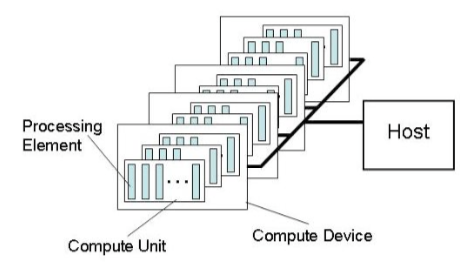
\includegraphics[width=0.4\textwidth]{figures/PlatformModel.png}
    \caption{Platform Model\cite{opencl12}.}
    \label{PlatformModel}
\end{figure}


\subsection{Memory Model}
\input{MemModel}
%------------------------------------------------
\section{OpenCL Mapping}
\par{This section will the most important features of the different architecture that we used for this work, it also explains the 
    mapping of the main OpenCL concepts into these different hardware architectures, also it will explain the most important 
    considerations of the OpenCL's \emph{kernel} execution into these devices}.

\subsection{Vectorization(Xeon and Xeon Phi)}
\par{On the Xeon and Xeon Phi architectures from Intel, to take advantage of these architecture, vectorization is compulsary.
    The OpenCL compiler provided by Intel, rewrites scalar and explicitly vectorized(Intel documentation firmly 
    advice against writing vector code using OpenCL vector types) kernel code into SIMD code. Intel documentation,
    does not explain the type of transformations that the compiler does to the code to vectorize it, which is a 
    problem when as programmers we want to track performance of OpenCL kernels.}

\par{Normally, to vectorize a loop(if dependencies do not exist), the loop is strip mined\footnote{Strip mining 
    transforms a singly nested loop into a doubly nested one, where the step of the outer loop is determined by for example
    vector length\cite{loops}.} by the vector length and then every scalar instruction in the loop is replaced by its 
    vector equivalent\cite{vector}.}

\par{As far as we know there are 2 types of vector transformations that the compiler can do over \emph{work items}(given
    that \emph{work items} are the basic unit of computation in OpenCL) to use vector units.}

\begin{itemize}
    \item Vectorization inside of a \emph{Work Item}, it is basically loop unrolling by a factor equal to the vector lenght of the
    architecture(16 for single precision on the Xeon Phi) then transforming the scalar instructions to vector instructions.

    \item Vectorization merging \emph{Work Items}, this vectorization is across \emph{work items} merging them making them 
    ``wider", and because of this reducing the number of \emph{work items} initially lunched by the 
    \emph{NDRange} call by a factor equal to the vector length of the architecture.
\end{itemize}

\par{This approaches can be applied together to OpenCL \emph{kernels}, although there are kernels that benefit better from 
    only one of this 2 approaches\cite{vector}.}
    





\subsection{CPU (Xeon)}
\label{sec:cpu}
\par{Table \ref{tab:xeon_arch} contains the main hardware characteristics of the Xeon CPU installed in fionn.}

\begin{table}[!h]
    \centering
    \begin{tabular}{| l | l | l | l |}
    \hline
    \# cores / socket& 10(out-of-order) \\ \hline
    \# threads / core& 2 \\ \hline
    \# sockets & 2 \\ \hline
    clock speed & 2.2 GHz \\ \hline
    typr & Ivy Bridge \\ \hline
    vector unit & 256-bit AVX \\ \hline
    L1 / core & 32KB(data)+32KB(instructions) 64KB total \\ \hline
    L2 / core & 256KB \\ \hline
    L3 /socket & 25MB \\ \hline
    \end{tabular}
    \caption{Xeon characteristics\cite{xeon_specs}.}
    \label{tab:xeon_arch}
\end{table}

\subsubsection{Mapping}

\par{The mapping of OpenCL concepts to Hardware are the same that in the Xeon Phi, see section \ref{sec:phi}.}

\par{{\color{red} PUT THE PICTURE OF THE OUTPUT OF DEVICEINFO AND PUT SOME COMMENTS ON IT!!!!!!}}

\subsection{Xeon Phi}
\label{sec:phi}
\subsubsection{Architecture}
\begin{itemize}
    \item 60 cores, In-order\cite{phi_specs}.
    \item 1.053 GHz of clock speed per core\cite{phi_specs}.
    \item Every core contains a 512-bit vector arithmetic unit(executing SIMD vector instructions). It fits 8 double precision 
        floating point numbers, or 16 single precision floating point numbers. Each core can issue a single vector instruction per
        cycle\cite{opencl_phi}(this execution looks similar to an Nvidia GPU \emph{warp}), so vector instructions issued by 
        different threads in the same core are sequentialized, they do not execute in parallel(at the same cycle).
    \item Each core has a L1 cache memory of 32KB for data and 32KB for instructions(64KB total). Miss latency 15-30
        cycles and access to L1 cache has a latency of 1 cycle\cite{opencl_phi}.
    \item Each core has a L2 cache of 512KB between data and instructions(combined 30MB of L2 cache). Miss latency 500-1000 cycles
        \cite{opencl_phi,phi_specs}.
    \item High speed interconect between L2 caches and the memory subsystem\cite{opencl_phi}.
    \item Simple automatic hardware prefetcher to L2\cite{opencl_phi}.
    \item Each core can execute 4 hardware threads simultaneously, 240 threads in total. These threads help to hide 
        instruction and memory latency\cite{opencl_phi}.
\end{itemize}

\par{OpenCL hides most of this detail from the programmer, figure \ref{PhiArch} shows a global view of the Intel Xeon Phi 
    architecture.\cite{opencl_phi}}

\begin{figure}[!h]
    \centering
    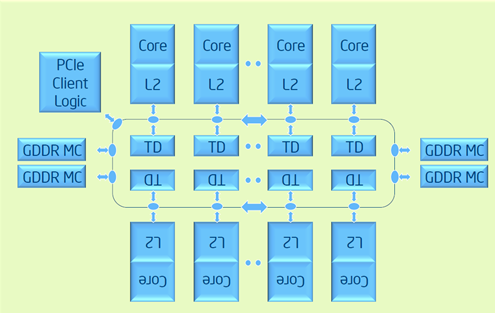
\includegraphics[width=0.6\textwidth]{figures/phi_arch.png}
    \caption{Intel Xeon Phi architecture\cite{opencl_phi}.}
    \label{PhiArch}
\end{figure}

\subsubsection{Mapping}
\begin{itemize}
    \item A \emph{work group} is the smallest task being scheduled on the threads\cite{opencl_phi}.
    \item \emph{Kernels} execute concurrently on multiple \emph{work items} in the SIMD units of every core\cite{opencl_phi_opt}.
    \item Each \emph{work group} is assigned to one thread that loops over all \emph{work items} within the \emph{work group} 
        with SIMD. So you have parallelism at the \emph{work group} level (vector instructions) and parallelism between 
        \emph{work groups} (threading)\cite{opencl_phi_opt}.
    \item At initialization time the Intel OpenCL driver creates 240 software threads and pins them to the hardware threads, then
        when you call \emph{clEnqueueNDRange()}, the intel driver schedules the \emph{work groups} of the current \emph{NDRange}
        into the 240 threads\cite{opencl_phi}.
    \item The OpenCL compiler implicitely vectorize the \emph{work group} routine based on dimension zero loop.
    \item The recommended work-group size for kernels is multiple of 16, which equals the SIMD width for the float and int data 
        type. The automatic vectorization module packs the work-items into SIMD packets of 16 items (for double as well), and 
        processed the rest (“tail”) of the work-group in a scalar way. In other words, a work-group with the size of 2*SIMD\_WIDTH 
        executes faster than, the one with the size of 2* SIMD\_WIDTH-1\cite{opencl_phi_opt,opencl_phi}.
    \item Non-uniform branching at dimension 0 the \emph{NDRange} is executed by flattening the code via predication and 
        ultimatelly executing both path of the branch and then apply masks, thus the usage of non-uniform branching is penalized by 
        a high overhead in the execution of the \emph{kernel}\cite{opencl_phi}.
    \item Using OpenCL \emph{local memory} does not provide any benefit on the Intel Xeon Phi. OpenCL \emph{local memory} is 
        allocated on the regular GDDR memory(\emph{global memory}) and is supported by the cache system like any other memory. 
        Therefore, it introduces additional overhead in terms of redundant data copy and management\cite{opencl_phi}.
    \item The combination of \emph{kernel} with barriers and \emph{work groups} nondivisible by 16, results in the execution of a
        scalar \emph{kernel}.
\end{itemize}

\begin{figure}[!h]
    \centering
    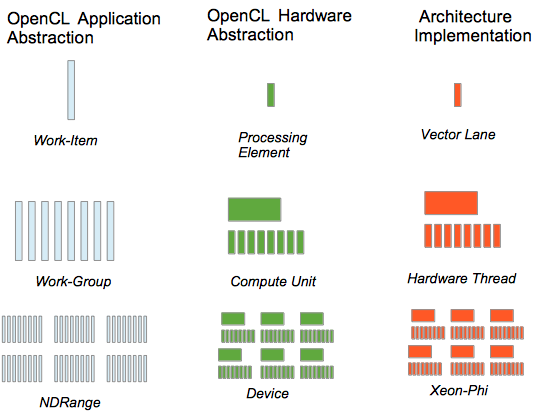
\includegraphics[width=0.7\textwidth]{figures/phi_model.png}
    \caption{OpenCL mapping for Intel Xeon Phi.}
    \label{PhiModel}
\end{figure}

\par{Figure \ref{PhiModel} shows a summary of the mapping of OpenCL concepts into the Intel Xeon Phi co-processor, figure 
    \ref{PhiDeviceInfo} shows the output of an OpenCL information request to the OpenCL run-time, it shows 236 
    \emph{compute units}(one per thread), the size of \emph{local memory} 32KB that match with the total amount of memory for L1 cache and
    the 6GB of total \emph{global memory} that matches with the amount of RAM available on the Intel Xeon Phi. In this context is 
    safe to assume that private memory on the Intel Xeon Phi is implemented via hardware registers.} 

\begin{figure}[!h]
    \centering
    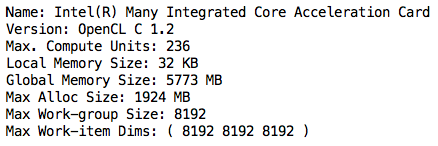
\includegraphics[width=0.7\textwidth]{figures/phi_device_info.png}
    \caption{Intel Xeon Phi device information.}
    \label{PhiDeviceInfo}
\end{figure}




\subsection{GPU}
\par{...}






\subsection{FPGA}
\par{...}


%------------------------------------------------
\section{Matrix Multiplication}
\par{To start this report we chose to analize the behaviour and performance of a Matrix Matrix multiplication algorithm 
    implementation, this is because this particular algorithm can be found in several scientific and HPC codes in several flavours
    and in its basic and more naive flavour is simple enough to be able to focus in OpenCL and the devices where is going to be 
    executed rather than the algorithm itself.}


\subsection{Naive}
\label{sec:naive}
\par{This implementation of this \emph{kernel} is as far as we know, the most 
    straightforward implementation of the matrix multiplication algorithm. 
    Optimisations were not implemented on this kernels as it can be seen in 
    listing \ref{naive_kernel}.} 
    
\par{Every instance of the \emph{kernel} calculates one element of the output 
    matrix(line 8), the \emph{NDRange} call is in 2 dimensions and all the 
    memory used for output and input data is global, this \emph{kernel}
    does not force caching or register usage via \emph{local} or \emph{private} 
    memory.}

\par{The results executing this kernel in different architectures with different 
    \emph{work group} dimensions can be seen in figure \ref{Naive}. From these 
    figures we can notice immediately that using dimensions greater than or 
    equal than 16 \emph{work items} in dimension 0 decreases the execution time 
    of the \emph{kernel} roughly 8 times in the case of Intel Xeon Phi. The
    Xeon CPU shows the same trend when the size of dimension 0 is greater or 
    equal than 2 but with an smaller decrease in execution time, 
    3.5 times approximately.}

\begin{figure}[!h]
    \centering
    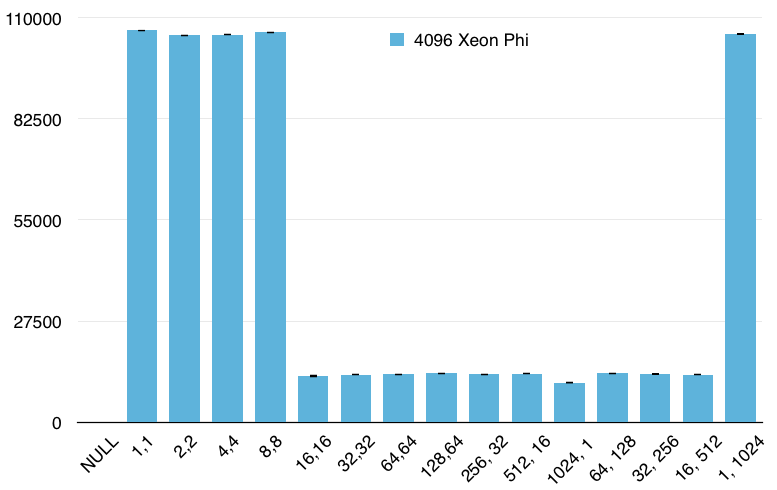
\includegraphics[width=0.49\textwidth]{figures/naive_phi.png}
    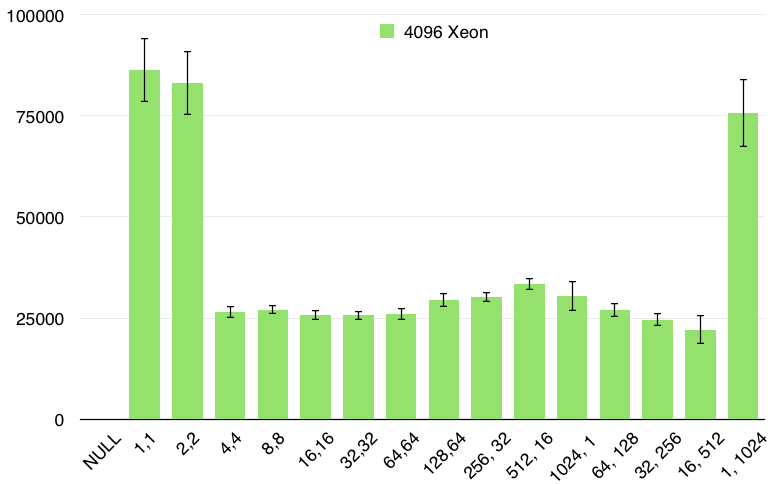
\includegraphics[width=0.49\textwidth]{figures/naive_cpu.png}
    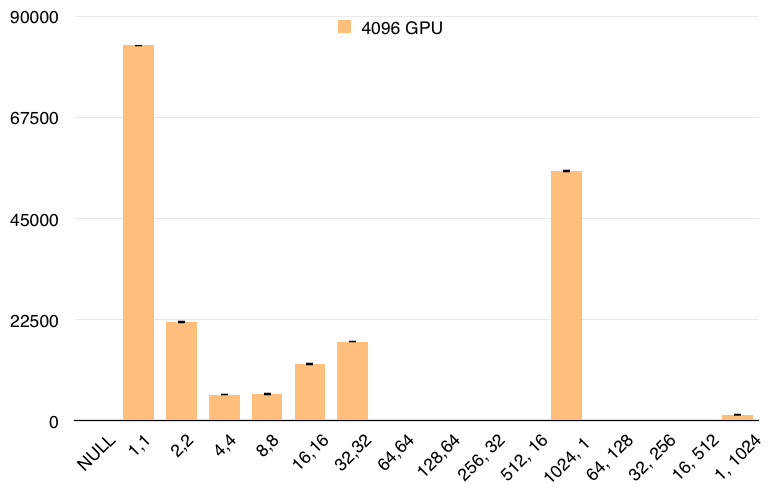
\includegraphics[width=0.49\textwidth]{figures/naive_gpu.png}
    \caption{Naive matrix multiplication results in different architectures.}
    \label{Naive}
\end{figure}

\par{Looking at listing \ref{llvm_code_naive_phi} we can realise that the 
    instructions that the Intel OpenCL compiler is generating are using a vector
    width of 16. This can explain the behaviour described previously and seen in
    figure \ref{Naive} for the Xeon Phi, being the \emph{work item} the basic 
    unit of computation in OpenCL, a \emph{work group} needs to have 16 \emph{
    work items} at least at dimension 0 to be able to use the entire width
    of the vector units available in the Xeon Phi. It seems that with numbers 
    less than 16 \emph{work items} inside of a \emph{work group} these 
    get serialized execution(using just one lane of the 16 available in the 
    vector registers of the Xeon Phi).}

\lstinputlisting[float,caption={Naive kernel LLVM code Intel Xeon Phi.}, 
    label={llvm_code_naive_phi}, 
    style=customc]
    {/Users/clalanne/GitHubProjects/OpenCLNotes/src/code/llvm_naive_phi.ll}

\par{Listing \ref{llvm_code_naive_cpu} and figure \ref{Naive} show the same 
    behaviour in the Xeon CPU, but with vector width of 4 instead of 16. Thus 
    in this case the Xeon CPU only needs 4 \emph{work items} at dimension 0
    of a \emph{work group} for the vectorization start to work. One intesting
    thing to notice is that the Xeon CPU has hardware support for AVX 
    vectorization, this means that the vector width should be of 256 bits, 
    available to fit 8 single precision numbers. We can se that even though 
    the Xeon CPU has support for AVX still the Intel OpenCL compiler generates
    by default instruction using just half of the vector width available.}

\lstinputlisting[float,caption={Naive kernel LLVM code Xeon.}, 
    label={llvm_code_naive_cpu}, 
    style=customc]
    {/Users/clalanne/GitHubProjects/OpenCLNotes/src/code/llvm_naive_cpu.ll}

\par{The way in which this \emph{kernel} is implemented, it shows poor data reuse
    forcing the system to request the data needed for computation from 
    \emph{global memory} using in a very inefficient way the cache system. 
    Figure \ref{vtune_naive} shows the profile of an execution of this \emph{
    kernel}, its possible to see the huge difference between the time that the
    \emph{kernel} spend bringing data from memory rather than using the data for
    computation(vgatherdps\footnote{Gather 2/4 packed 
    single-precision floating point values from memory referenced by the given 
    base address, dword indices and scale\cite{intrinsics}}
    \footnote{vgatherdps works by getting the data cache linewise per 
    invocation; this means that every time the gather instruction 
    is used, it will fetch only one cache line (CL), load all the values that 
    it is supposed to gather from it, store them in 
    the destination vector register, and finally zero out the bits of the 
    components that have been filled in the vector mask 
    register. As a consequence, the number of gather instruction depends on 
    the distribution of the data: 
    If all data resides in one CL then one gather instruction is sufficient; 
    in the worst case, each value is located in a different CL, 
    which will require sixteen gather instructions\cite{simd}.} vs vfmadd231ps).}

\begin{figure}[!h]
    \centering
    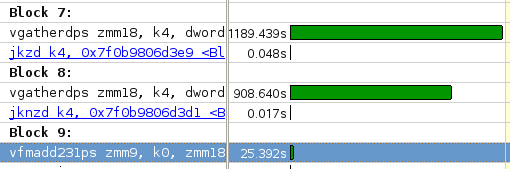
\includegraphics[width=0.49\textwidth]{figures/vtune_naive.png}
    \caption{Vtune profiler in the native kernel.}
    \label{vtune_naive}
\end{figure}

\par{{\color{red}Reading the listing \ref{naive_kernel}, its possible to see that there is no effort to use caches efficiently, the locality of
    memory access pattern its far from ideal. At the top of this, the gathering of data from memory results in having a high CPI(clock per
    instructions)\footnote{The CPI value of an application or function is an indication of how much latency affected its execution. 
    Higher CPI values mean there was more latency in your system – on average, it took more clockticks for an instruction to retire. 
    Latency in your system can be caused by cache misses, I/O, or other bottlenecks\cite{cpi}.} 
    rate poor vectorization and low L1 hit ratio for this kernel on the Xeon and Xeon Phi.}}

\par{For the GPU figure \ref{Naive} shows that not in all of the 
    \emph{work group} dimensions is possible to execute the kernel. 
    This is because the GPU run out of resources in those cases\cite{opencl_error},
    figure \ref{GpuDeviceInfo} and table \ref{tab:gpu_arch} show that the 
    maximum number of \emph{work group} size is of 1024 \emph{work items} which
    is exceeded by several of the \emph{work group} dimensions shown in figure 
    \ref{Naive}(\emph{e.g. 64x64}).}

\par{Figure \ref{NaiveRes} shows that GPUs achived the best performance in 
    comparison with the other architectures particularly
    in the case where the \emph{work group} dimension is 1x1024,
    this is mainly because the memory access patterns to access matrix A and B. 
    Access to matrix B its coalesced which means that the GPU can combine several 
    memory accesses into a single transaction, the memory access pattern for matrix 
    A also can be optimised, all the \emph{work items} in a warp access(read only)
    to the same memory space}.

\begin{figure}[!h]
    \centering
    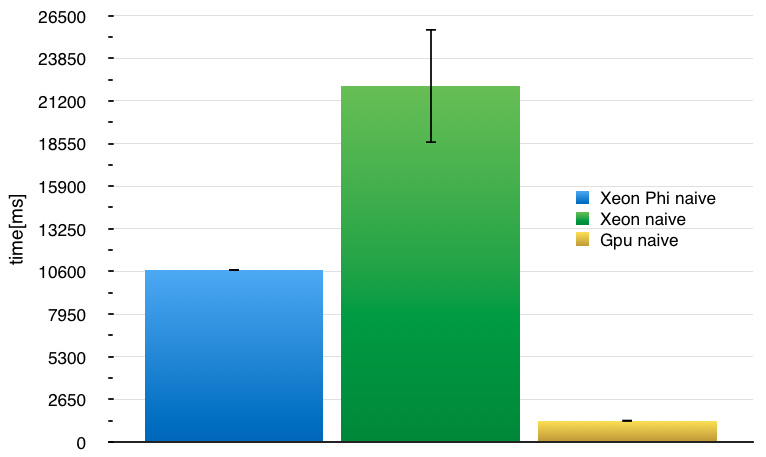
\includegraphics[width=0.49\textwidth]{figures/naiveRes.png}
    \caption{Comparison between the best cases in the different devices.}
    \label{NaiveRes}
\end{figure}

\par{Using warps and lock-step execution for the 
    GPU and vectorization of \emph{work items} for the Xeon and Xeon Phi, both
    memory access patterns are similar, with the difference that if we look at
    the GPU as a vector processor(warp execution) with double of the width that the
    Xeon Phi vector unit we can explain the better performance that this device 
    has against both Intel processors.}




\subsection{More Work}
\label{sec:moreWork}
\par{...\ref{MoreWork}\ref{MoreWorkComp}}

\begin{figure}[!h]
    \centering
    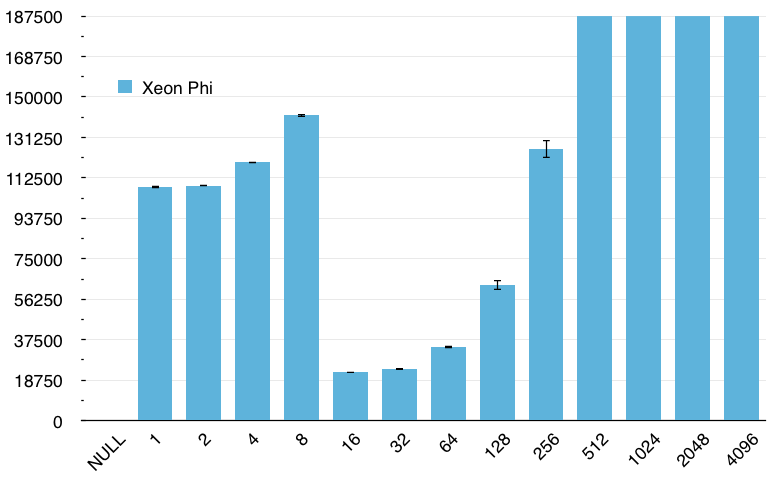
\includegraphics[width=0.49\textwidth]{figures/opt1_phi.png}
    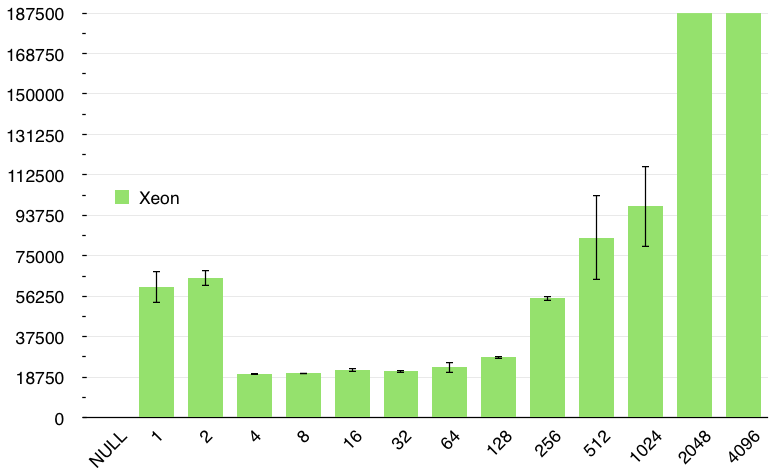
\includegraphics[width=0.49\textwidth]{figures/opt1_cpu.png}
    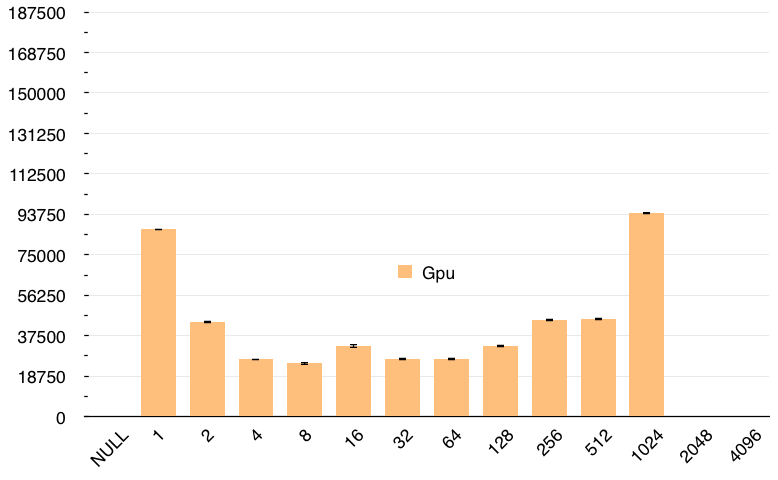
\includegraphics[width=0.49\textwidth]{figures/opt1_gpu.png}
    \caption{Matrix multiplication with more work in different architectures.}
    \label{MoreWork}
\end{figure}

\begin{figure}[!h]
    \centering
    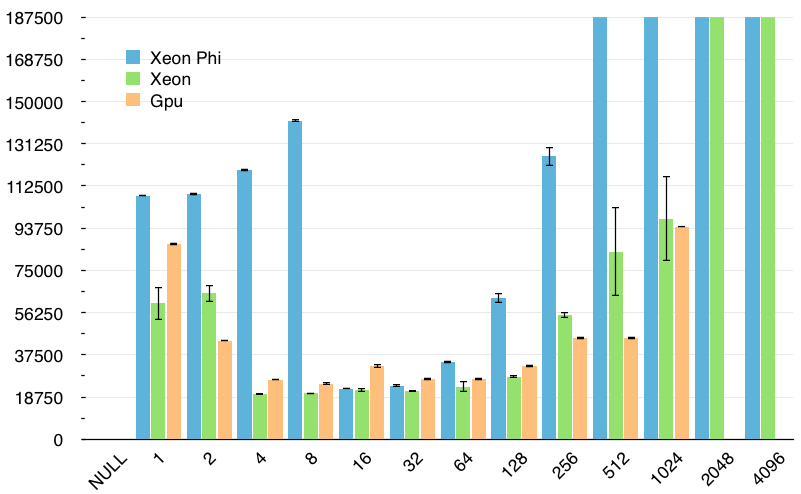
\includegraphics[width=0.6\textwidth]{figures/opt1_comp.png}
    \caption{Matrix multiplication with more work in different architectures comparison.}
    \label{MoreWorkComp}
\end{figure}


\subsection{Rows}
\label{sec:rows}
\par{...}

\subsection{Rows and Columns}
\label{sec:rowscols}

\par{Listing \ref{private_local_memory_kernel} shows the kernel that uses together \emph{private memory} to bring elements of A to 
    on-chip memory and \emph{local memory} to cache column B. In 
    this case the amount of \emph{local memory} to use is passed to the kernel as the fourth argument. The main idea for this is
    that all work items share the same column of B to avoid going into \emph{global memory}.}

\par{As in the previous kernel line \emph{12} shows the copy of elements to \emph{private memory} and line \emph{15} shows the 
    copy of elements from \emph{global memory} to \emph{local memory}, also ...\emph{expand on the use of barriers}.}

\lstinputlisting[float,caption={Kernel making use of \emph{private memory} and \emph{local memory}.},label={private_local_memory_kernel}, 
                style=customc]{/Users/clalanne/GitHubProjects/OpenCLNotes/src/code/private_local_memory.c}

\par{Figure \ref{RowsCols} shows the results of this kernel for different architectures, not all \emph{work group} dimensions 
    were possible to execute for this \emph{kernel}. For the case of the Xeon and Xeon Phi from the 32x32 the runtime returned
    error -5, that means was a failure to allocate resources\cite{opencl_error}, this mainly is because we are forcing to the 
    allocation of local memory ~16KB per \emph{work item}.

\begin{figure}[!h]
    \centering
    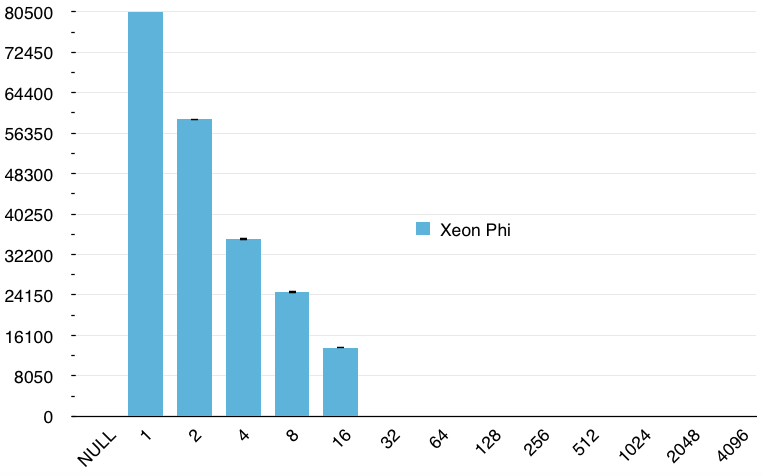
\includegraphics[width=0.49\textwidth]{figures/opt3_phi.png}
    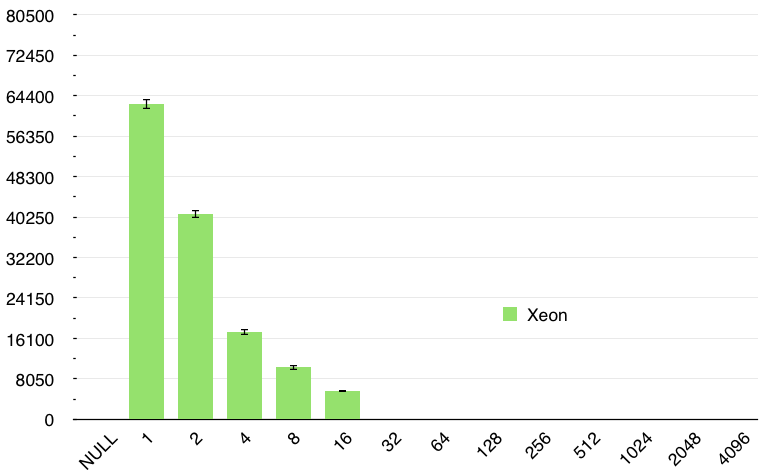
\includegraphics[width=0.49\textwidth]{figures/opt3_cpu.png}
    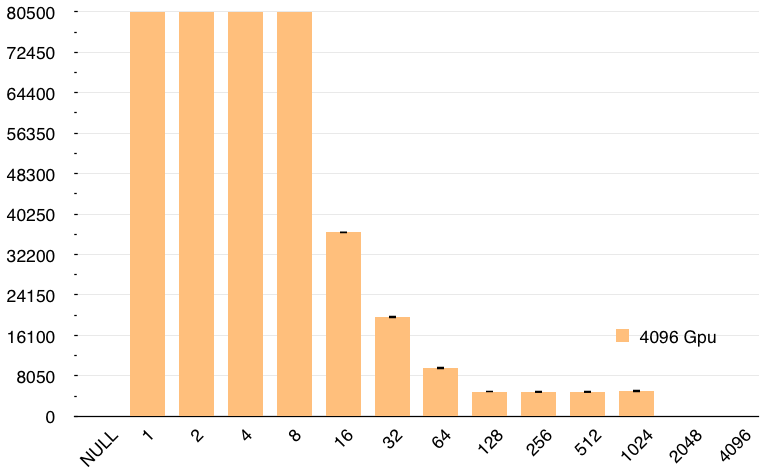
\includegraphics[width=0.49\textwidth]{figures/opt3_gpu.png}
    \caption{Rows and columns optimisation matrix multiplication in different architectures.}
    \label{RowsCols}
\end{figure}

\par{It seems to be a trade off here, between the the loop necesary to execute the copy of elements of B to \emph{local memory}
    (expensive gathering operations with a very poor L1 hit ratio) and the performance achieve in the loop where the kernel executes
    the computation(\emph{maybe vtune shot}).}

\par{In this case the best time is achived again by the GPU as we can see in figure \ref{RowsColsComp}, Also we can notice that the only 
    architectures that is able to take advantage of this optimisation is the Xeon. The Xeon Phi even have a warning in its 
    documentation about not using \emph{local} memory explicitelly as in this case, because of the cache system already is using 
    automatically this memory, and even warn about possible overhead time if this memory is defined explicitely\cite{opencl_phi}.}

\begin{figure}[!h]
    \centering
    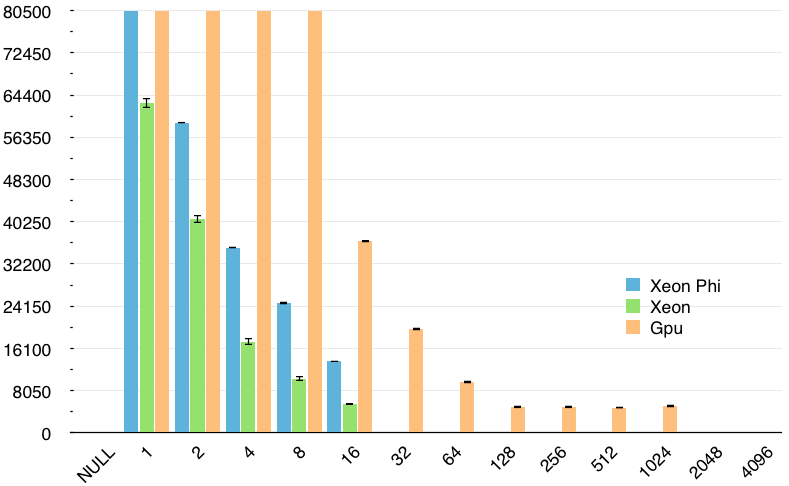
\includegraphics[width=0.6\textwidth]{figures/opt3_comp.png}
    \caption{Rows and columns optimisation matrix multiplication with more work in different architectures comparison.}
    \label{RowsColsComp}
\end{figure}


\subsection{Tiling}
\label{sec:tiling}
\par{...}

%------------------------------------------------
\section{LU Descomposition}
\par{The performance of OpenCL was studied using an implementation of 
    the LU decomposition algorithm. This algorithm is computationally intense, 
    with a high number of algebraic operations compared to the size of the data. 
    Due to the susceptibility of the LU decomposition to round-off errors, 
    matrices of double-precision floating point numbers were used.}

\subsection{Algorithm Overview}
\par{This OpenCL implementation of the LU decomposition was done with three 
    separate \emph{kernels}. Each of these \emph{kernels} performed operations on different 
    areas of a NxN matrix and the \emph{kernels} were enqueued multiple times.}

\par{A key parameter in this algorithm is the block size, which is defined 
    both in the host and \emph{kernel} code. It can take values of 2, 4, 8, 16, 32 
    and 64. A block size of 64 is not supported on the GPU, due to \emph{work group} 
    size restrictions. The value of the block size is not changed during the 
    computation. The block size explicitly determines a number of variables, 
    including the number of \emph{work groups}, the number of \emph{work items} per 
    \emph{work group}, the size of the data block and the number of times the 
    \emph{kernels} are enqueued. It is also important to note that the overall number of 
    floating point operations required to compute the LU decomposition varies 
    according to the block size.}


\par{The three \emph{kernels} are enqueued at each iteration of a for loop in the 
    host code, with various parameters such as the number of \emph{work groups}, 
    number of \emph{work items} and data size changing at each iteration of the 
    loop.}


\subsubsection{Diagonal Kernel}
\par{As the name suggests, the diagonal kernel performs operations on the diagonal elements of the matrix. 
    Table \ref{tab:lu1} summarises how the block size affects the implementation of the diagonal kernel.}

\begin{table}[!h]
    \centering
    \begin{tabular}{| l | l | l | l |}
    \hline
    \emph{Block Size} & \emph{Data Block} & \emph{\#Work Groups} & \emph{\#Work-Items / Work-Group} \\ \hline
    2 & 2x2 & 1 & 2 \\ \hline
    4 & 4x4 & 1 & 4 \\ \hline
    8 & 8x8 & 1 & 8 \\ \hline
    16 & 16x16 & 1 & 16 \\ \hline
    32 & 32x32 & 1 & 32 \\ \hline
    64 & 64x64 & 1 & 64\\ \hline
    \end{tabular}
    \caption{rory blah blah.}
    \label{tab:lu1}
\end{table}

\par{The first point to note is that the diagonal kernel is clearly not optimised for parallel computing. 
    In OpenCL, the work-groups are scheduled in parallel on each thread of the Xeon Phi and Xeon CPU. 
    In this case, the number of work-groups is always one. For example, on the Xeon Phi, 
    the entire computation of the diagonal kernel would take place on just one of the 240 hardware threads.}

\par{Although there is no parallelism between threads in this case, implicit SIMD vectorisation of work-items is supported 
    by the OpenCL compiler. However, this requires both that kernels be as simple as possible and that they execute the same 
    instructions. This is not the case with this kernel. The algorithm is such that each work-item carries out a different 
    number of floating point operations, depending on its ID. This renders instruction-level parallelism impossible in this case. 
    Figure \ref{FlopCount} shows that, for a work-group of 16 work-items, the number of floating point operations varies according to 
    the ID of the work-item. In fact, the first work-item of every work-group does no computation whatsoever.}

\begin{figure}[!h]
    \centering
    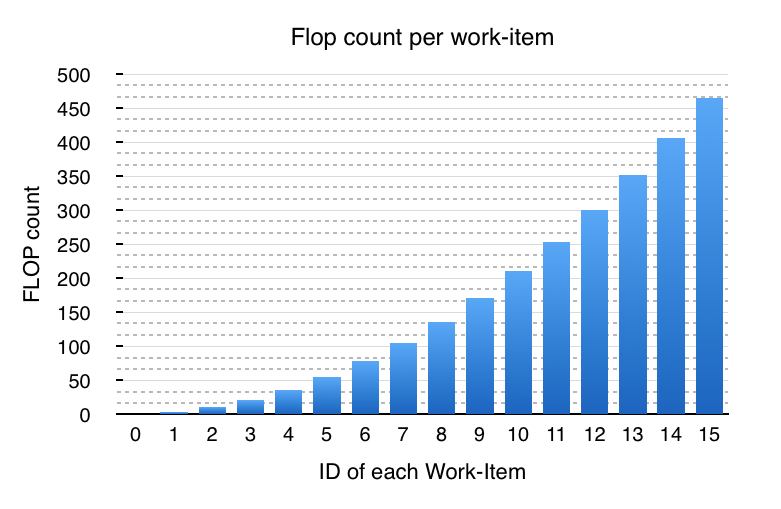
\includegraphics[width=0.6\textwidth]{figures/FlopCount.png}
    \caption{Rory blah blah blah.}
    \label{FlopCount}
\end{figure}

\par{Figure \ref{DiagonalKernel} illustrates a number of important points. It is clear that, 
    out of the three devices used, the Xeon Phi shows the worst performance. 
    Achieving high-performance with the Xeon Phi requires that work-items be vectorised and 
    that large numbers of work-groups be scheduled in parallel. Neither such condition is satisfied in this case. 
    It is interesting to note that the Xeon CPU performs best with an algorithm of low parallelism. 
    Undoubtedly, the CPU’s support for out-of-order execution gives it an advantage over the Xeon Phi, 
    which supports in-order execution only.}

\begin{figure}[!h]
    \centering
    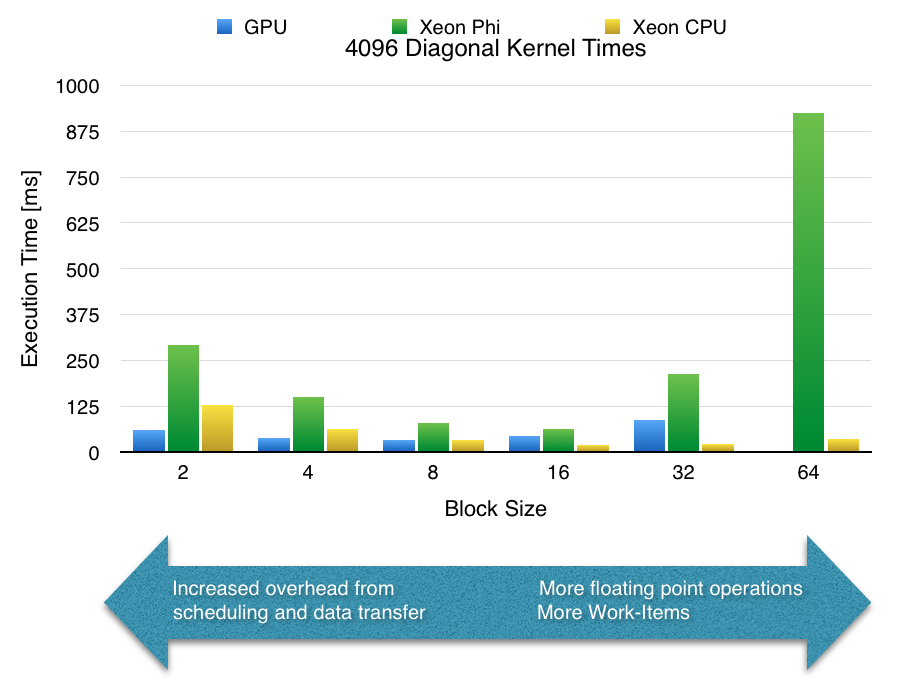
\includegraphics[width=0.6\textwidth]{figures/DiagonalKernel.png}
    \caption{Rory blah blah blah.}
    \label{DiagonalKernel}
\end{figure}

\par{The GPU also achieves good performance compared to the Xeon Phi. Unlike on the Xeon CPU and Xeon Phi, 
    the work-items are scheduled in parallel in the warps of the GPU. It does not suffer the same lack of 
    performance as a result of having only 1 work-group.}




\subsubsection{Perimeter Kernel}
\par{The perimeter kernel, despite what its name suggests, does not necessarily operate on elements 
    at the perimeter of the matrix. Figure \ref{PerimeterKernel2} demonstrates the areas of the matrix where the 
    perimeter kernel computes.}

\begin{figure}[!h]
    \centering
    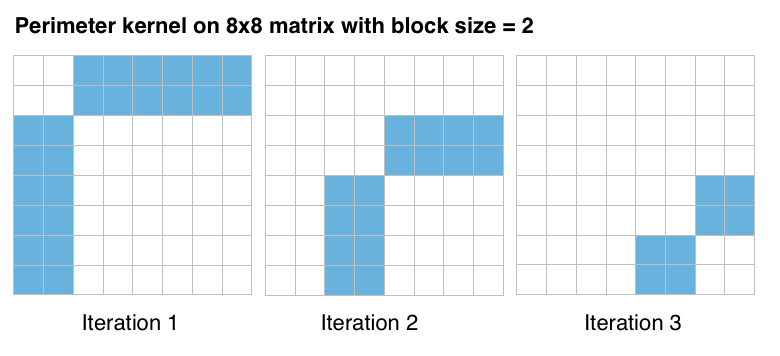
\includegraphics[width=0.6\textwidth]{figures/PerimeterKernel2.png}
    \caption{Rory blah blah blah.}
    \label{PerimeterKernel2}
\end{figure}

\par{This kernel, like the other two kernels, is enqueued multiple times by the host, each 
    time to operate on a different portion of the matrix, as shown above.}

\par{At each iteration of the loop in the host code, the total number of work-groups is decreased by one. 
    Eventually, in the last iteration of the loop, only 1 work-group will be enqueued. 
    Since work-groups are scheduled in parallel on the Xeon Phi and Xeon CPU, 
    this means that the parallelism of the algorithm reduces as the computation proceeds.}

\par{The opposite is true for the GPU. The number of work-items per work-group increases for greater block sizes. 
    This increases the parallelism of the algorithm on the GPU. In both cases, however, 
    there is guaranteed to be at least some under-utilisation of the hardware threads. 
    Table \ref{tab:lu2} summarises some of the relevant parameters.}

\begin{table}[!h]
    \centering
    \begin{tabular}{| l | l | l | l |}
    \hline
    \emph{Block Size} & \emph{Data Size / Work Group} & \emph{Starting Number of Work Groups} & \emph{\#Work-Items / Work-Group} \\ \hline
    2 & 2x2 & 2047 & 4 \\ \hline
    4 & 4x4 & 1023 & 8 \\ \hline
    8 & 8x8 & 511 & 16 \\ \hline
    16 & 16x16 & 255 & 32 \\ \hline
    32 & 32x32 & 127 & 64 \\ \hline
    64 & 64x64 & 63 & 128 \\ \hline
    \end{tabular}
    \caption{rory blah blah.}
    \label{tab:lu2}
\end{table}

\par{The performance of this kernel can be explained as a compromise between a number of parameter changes. 
    Firstly, a greater block size will decrease the number of work-groups and increase the number of work-items per work-group. 
    For example, with a block size of 32, there will be a maximum of 127 work groups, 
    reducing to 1 work-group as the computation proceeds, but there will be 64 work-items per work-group. 
    In this case, the algorithm would be under-utilising the hardware threads of the Xeon CPU and the Xeon Phi, 
    but exploiting the parallelism available in the GPU.}

\par{A greater block size reduces the overhead of loading data from global to local memory, 
    since more data is loaded to memory at each execution. For each greater block size, 
    the total number of floating-point operations approximately doubles.}

\begin{figure}[!h]
    \centering
    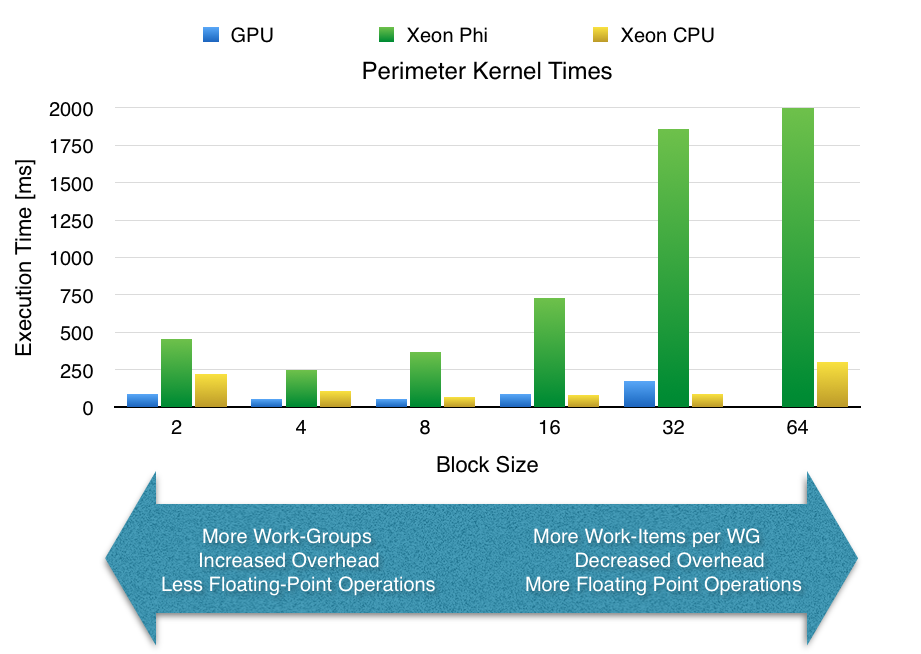
\includegraphics[width=0.6\textwidth]{figures/PerimeterKernel1.png}
    \caption{Rory blah blah blah.}
    \label{PerimeterKernel1}
\end{figure}

\par{Figure \ref{PerimeterKernel1} summarises these points. An increase in block size effectively 
    reduces the parallelism of the algorithm on the Xeon CPU and Xeon Phi, but reduces 
    the overhead incurred from high-latency data transfers. For the GPU, the increase 
    in block size gives rise to a higher level of parallelism, since work-items are scheduled 
    in parallel on the cores within each streaming multiprocessor. Unfortunately, the fact that the 
    total number of floating point operations increases according to the block size skews the results.}


\subsubsection{Internal Kernel}
\par{The internal kernel is the dominant kernel in this implementation of the LU decomposition. 
    It accounts for the majority of computation time. It operates on a larger amount of data 
    than each of the other kernels and is also very inefficient, in spite of a high level of parallelism.}

\begin{figure}[!h]
    \centering
    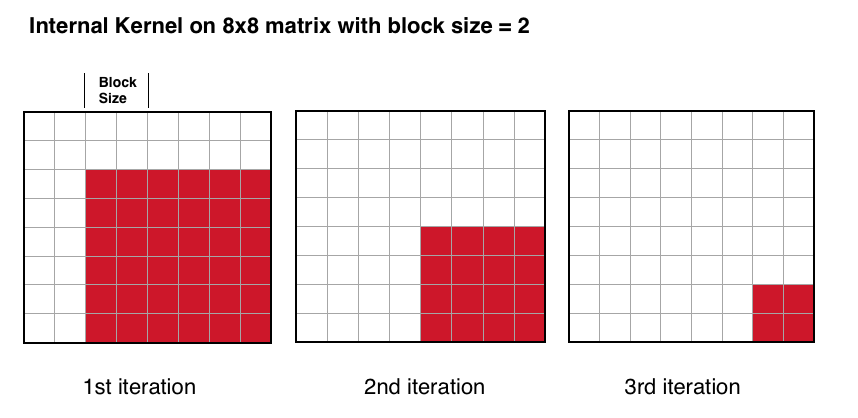
\includegraphics[width=0.6\textwidth]{figures/InternalKernel2.png}
    \caption{Rory blah blah blah.}
    \label{InternalKernel2}
\end{figure}

\par{The first instance of the internal kernel operates on the 1st portion of the matrix shown in figure \ref{InternalKernel2}. 
    All kernels are enqueued multiple times, so, the next execution of the kernel will operate on 
    a portion of the matrix that has been decreased by block size in each dimension.}

\par{Table \ref{tab:lu3} summarises the relevant parameters.}

\begin{table}[!h]
    \centering
    \begin{tabular}{| l | l | l | l |}
    \hline
    \emph{Block Size} & \emph{Data Block / Work Group} & \emph{Starting Number of Work Groups} & \emph{\#Work-Items / Work-Group} \\ \hline
    2 & 3x(2x2) & 4,190,209 & 4 \\ \hline
    4 & 3x(4x4) & 1,046,529 & 16 \\ \hline
    8 & 3x(8x8) & 261,121 & 64 \\ \hline
    16 & 3x(16x16) & 65,025 & 256 \\ \hline
    32 & 3x(32x32) & 16,129 & 1024 \\ \hline
    64 & 3x(64x64) & 3,969 & 4096 \\ \hline
    \end{tabular}
    \caption{rory blah blah.}
    \label{tab:lu3}
\end{table}

\par{The first thing to note is that the number of work-groups is very high, which means
    that the algorithm is exploiting the available parallelism in the Xeon CPU and Xeon Phi relatively well. 
    There are almost always enough work-groups to fill the available hardware threads. 
    As a result, the number of GFLOPS is significantly higher in executions of the internal 
    kernel than in executions of the other kernels, which do not exploit the parallelism to the same extent. 
    This is a clear demonstration of the performance gains possible from correct utilisation of the available hardware. 
    Table \ref{tab:lu4} compares the number of GFLOPS between executions of the diagonal 
    kernel and the internal kernel on the Xeon CPU.}

\begin{table}[!h]
    \centering
    \begin{tabular}{| l | l | l | l |}
    \hline
    \emph{Block Size} & \emph{Diagonal} & \emph{Internal} \\ \hline
    2 & 0.00005 & 8.40286 \\ \hline
    4 & 0.00057 & 16.53493 \\ \hline
    8 & 0.00172 & 26.83808 \\ \hline
    16 & 0.03334 & 29.94455 \\ \hline
    32 & 0.11905 & 28.50387 \\ \hline
    64 & 0.30937 & 26.86795 \\ \hline
    \end{tabular}
    \caption{Comparison of GFLOPS - Diagonal v Internal Kernels.}
    \label{tab:lu4}
\end{table}

\par{In spite of this, the internal kernel is clearly not an optimal algorithm. 
    When the work-groups are first enqueued, the kernels operate on a very large block of data. 
    In the next iteration of the loop, the kernels operate on almost the same block of data, 
    albeit decreased by block size in each dimension. Thus, the kernel is operating multiple times 
    on almost the same blocks of data. There is an enormous amount of time spent carrying out redundant 
    calculations and reloading the same data from global to local memory.}

\par{The total number of floating point operations that the internal kernel executions perform 
    reduces with the block size, since the number of redundant operations reduces.}

\par{Figure \ref{InternalKernel1} below shows the total computation times for the internal kernel on each of the three devices.}

\begin{figure}[!h]
    \centering
    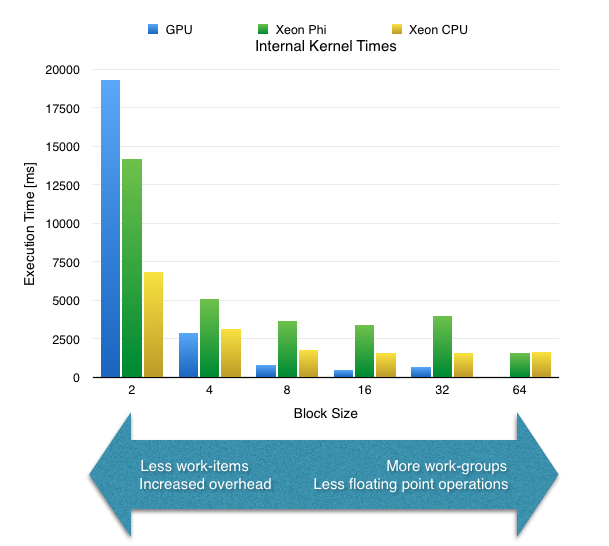
\includegraphics[width=0.6\textwidth]{figures/InternalKernel1.png}
    \caption{Rory blah blah blah.}
    \label{InternalKernel1}
\end{figure}

\par{The above graph highlights some interesting points. It is clear to see that when 
    the number of work-items is minimised (block size 2), the GPU offers the worst performance. 
    As mentioned previously, optimal performance on the GPU is achieved with a large number of 
    work-items per work-group. Significant performance improvements are seen on the GPU 
    as the number of work- items per work-group increases.}

\par{Another interesting point to note is that, as the block size increases, 
    the performance of the Xeon CPU and Xeon Phi improves. This is not only due 
    to the decrease in floating point operations, but also due to the increase in
    work-items per work-group whilst still maintaining a large number of work-groups. 
    Intel’s SDK for OpenCL Applications states that:}

\par{\emph{``To reduce the overhead of maintaining a work-group, create work-groups that
    are as large as possible. Still there should be a sufficient number of work-groups."}}

\par{The internal kernel satisfies these conditions for large block sizes and the performance improves as a result.}

%------------------------------------------------
\section{N-Body Methods}
\par{``N-body methods calculate interactions between many discrete points and are characterized 
    by large numbers of in- dependent calculations within a time step, followed by all-to- all 
    communication between time steps. Our GEM code calculates the effect that all atoms have on 
    the charge at each point along the surface of a molecule, leading to O(M ∗ N ) 
    complexity where N is atoms and M is points along the surface.”\cite{dwarfs}}

\par{For this particular N Body Problem, we are computing biomelcular electrostatic 
    surface potential. The calculation of potential is done using the linearized 
    Poisson-Boltzmann model (ALPB). This is implemented in the GEM package 
    (an open-source implementation of ALPB) . The potential at any single point in space, 
    for example a vertex point on the molecular surface, is computed as a sum of contributions 
    from the individual atomic charges in the solute.}

\par{Figure \ref{nbody} and equation \ref{eq:nbody} illustrates what is being calculated and the simplified ALPB equation 
    with which the calculation is performed.}

\begin{figure}[!h]
    \centering
    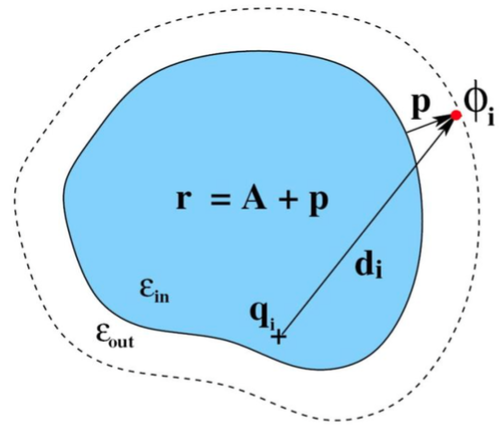
\includegraphics[width=0.5\textwidth]{figures/nbody.png}
    \caption{N-body problem.}
    \label{nbody}
\end{figure}

\begin{equation} \label{eq:nbody}
    \Phi_i^{solvent} = \frac{q_i}{\in_{out}}\frac{1}{(1+\alpha\frac{\in_{in}}{\in_{out}})}\Bigg[\frac{1+\alpha}{d_i}-\frac{\alpha(1-\frac{\in_in}{\in_out})}{r}\Bigg]
\end{equation}

\par{Where \Phi is electrostatic potential at point of interest/observation, \emph{qi} is the 
    electrostatic potential at point of interest/observation, \emph{di} is the distance from 
    the source charge qi to the point of observation, \alpha is a constant and \emph{r} is the 
    distance from the point of observation to the ``centre".}

\par{\emph{A} is the effective electrostatic size of the molecule and \emph{p} is the perpendicular 
    distance of the vertex point from the surface of the molecule.}

\par{The molecular surface(solid line) separates the low dielectric interior(\in in blue region) 
    from the high dielectric solvent space, \in out.}


\par{The method of Hierarchical Charge Partitioning(HCP)(figure \ref{hpc}) is also implemented within the code, 
    to allow for greater accuracy while also restricting the computational bottlenecks. 
    HCP exploits the natural partitioning of bio molecules into constituent structural components. 
    This use of multi-scale approximations for the potential allows for speed-ups to be achieved.}

\begin{figure}[!h]
    \centering
    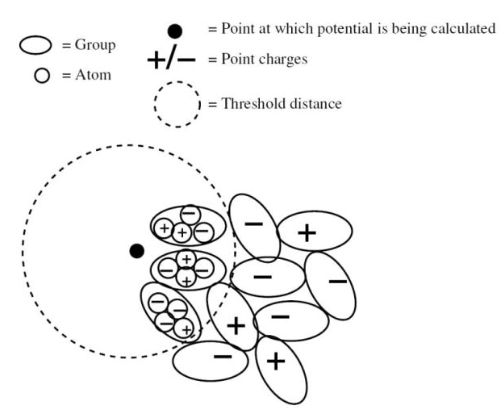
\includegraphics[width=0.5\textwidth]{figures/hpc.png}
    \caption{Hierarchical Charge Partitioning(HCP)\cite{nbody_gpu}.}
    \label{hpc}
\end{figure}

\par{The electrostatic effect of distant components is calculated from a small set of point charges. 
    Whereas, with nearby components, full sets of atomic charges are used for electrostatic interactions.}






\subsection{Implementation with OpenCL}
\par{Host code calls \emph{kernel} code multiple times based on the 
    number of global \emph{work items} declared and the number of vertices 
    on the surface of the selected bio molecule. There are 30 arguments 
    passed to the \emph{kernels}, with 16 of these being 
    \emph{\_\_global CL\_MEM\_READ\_ONLY}
    buffers and 1 being \emph{\_\_global CL\_MEM\_READ\_WRITE} buffer 
    for the final output. Pseudo code of the host is shown in listing 
    \ref{nbody_host}.}

\lstinputlisting[float,caption={Nbody host pseudo code.},label={nbody_host}, 
                style=customc]
                {/Users/lalanne/MyCode/GitHubProjects/OpenCLNotes/src/code/nbody_host.c}

\par{Every \emph{work item} in OpenCL is an implementation of the \emph{kernel} code. 
    Hence each \emph{work item} does a single step n body calculation. 
    i.e. Each \emph{work item} is working on the total electrostatic 
    potential on a vertex due to the atoms.}

\par{The \emph{kernel} code executes a regular computation pattern, 
    with each \emph{work item} per \emph{work group} performing the same computation. 
    This results in no dependencies that may hinder computation continuity. 
    Computations include divsion and square root operations on floating point 
    numbers which is an expensive bottleneck. Pseudo code of \emph{kernel} code
    is shown in listing \ref{nbody_kernel}.}

\lstinputlisting[float,caption={Nbody kernel pseudo code.},label={nbody_kernel}, 
                style=customc]
                {/Users/lalanne/MyCode/GitHubProjects/OpenCLNotes/src/code/nbody_kernel.c}

\par{Based on the processor in use, making changes to the \emph{work group} sizes 
    can greatly affect the efficiency and speed of the program. 
    As with any \emph{kernels}, optimising the code to fit the hardware is essential. 
    Understanding the hardware is an essential part of OpenCL 
    code development.}

\par{A ghraphical representation of the \emph{kernel} code is shown in figure 
    \ref{nbody_graph}.}

\begin{figure}[!h]
    \centering
    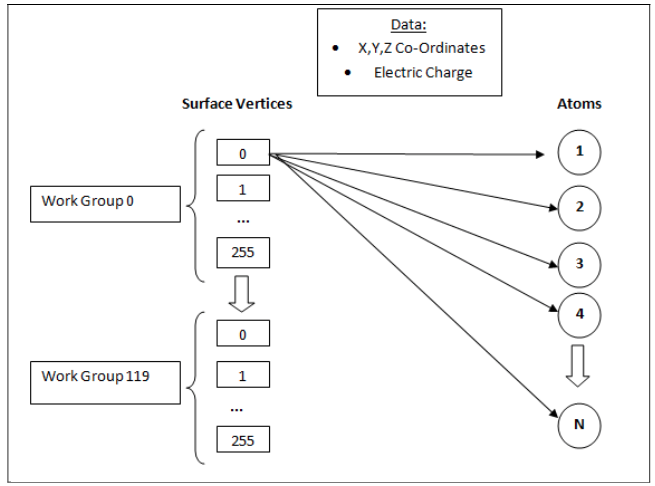
\includegraphics[width=0.5\textwidth]{figures/graph_nbody.png}
    \caption{Graphical representation of \emph{kernel} code.}
    \label{nbody_graph}
\end{figure}






\subsection{Graphical Trends}
\subsubsection{Xeon}
\par{Intel Xeon E5-2660 v2 (Ivy Bridge): Vector Arithmetic Unit with 256-bit 
    SIMD vectors.}

\par{The kernel is dealing with calculations on single precision 
    floating point. Each floating point number is of size 32 bits(4 byte). 
    Therefore there needs to be at least 8 work items in dimension 0 for 
    every work group. The hardware requires this in order to fully utilize 
    vectorization in the SIMD vector units. Any lower than this results 
    in under utilization of data parallelism, as can be seen clearly from 
    the graph trends of both capsid and nucleosome in figure \ref{nbody_xeon}.}

\begin{figure}[!h]
    \centering
    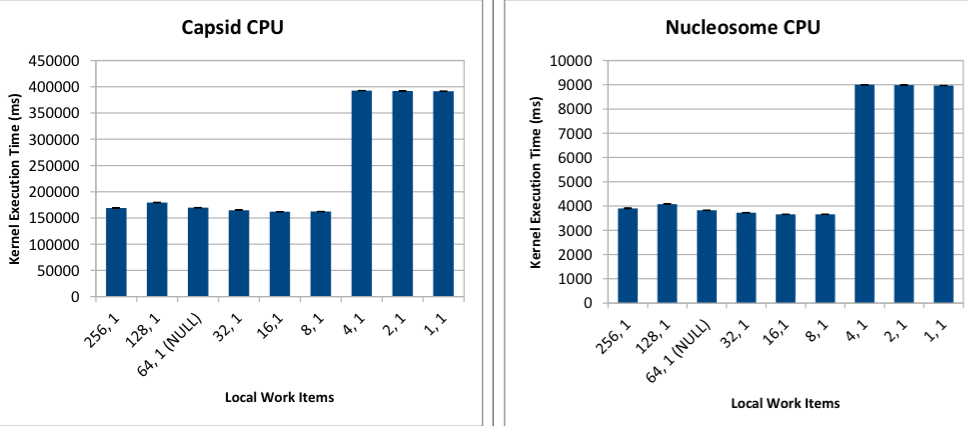
\includegraphics[width=0.8\textwidth]{figures/nbody_xeon.png}
    \caption{Graphical trends Nbody problem, Capsid and Nucleosome on Xeon.}
    \label{nbody_xeon}
\end{figure}

\par{From the profiler results in figure \ref{nbody_vtune}, 
    it is clear that this kernel is a good 
    fit for parallel computing. For the majority of the total run time, most 
    of the 40 cores are being used in the CPU. The small amount of time spent 
    with only 1 core running is likely due to the host and other code which 
    are required for this calculation.}

\begin{figure}[!h]
    \centering
    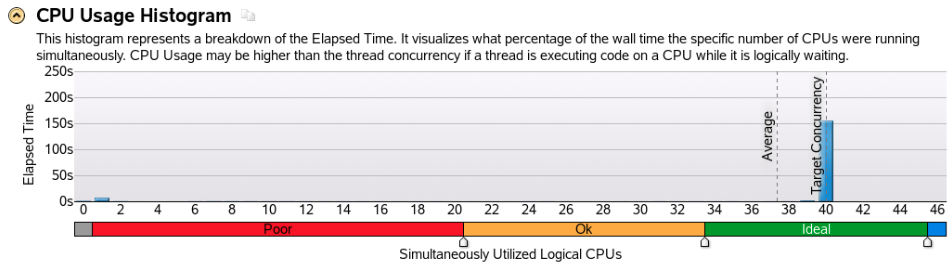
\includegraphics[width=0.8\textwidth]{figures/nbody_vtune.png}
    \caption{Vtune CPU usage histogram, nbody problem.}
    \label{nbody_vtune}
\end{figure}

\subsubsection{Xeon Phi}
\par{Intel Xeon Phi 5110P: Vector Arithmetic Unit with 512-bit SIMD vectors}

\par{The same logic can be applied to the Xeon Phi. The only 
    difference is that the Phi has larger vector units than the CPU. 
    Hence, there needs to be 16 work items in dimension 0 per work group. 
    This can be seen in figure \ref{nbody_phi}.}

\begin{figure}[!h]
    \centering
    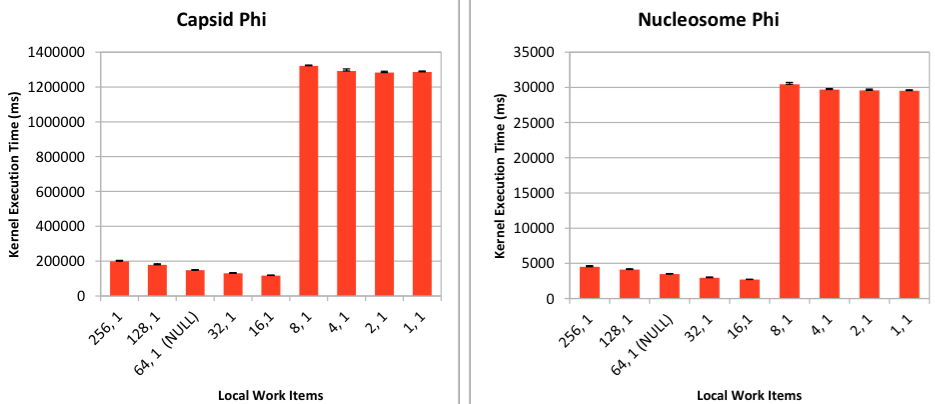
\includegraphics[width=0.8\textwidth]{figures/nbody_phi.png}
    \caption{Graphical trends Nbody problem, Capsid and Nucleosome on Xeon Phi.}
    \label{nbody_phi}
\end{figure}

\par{Figure \ref{nbody_phi_vec} clearly shows that the vector intensity with 16 work items 
    is the greatest. The same results must be occurring on the CPU as 
    we see a very similar trend in the graphs. 
    The high vectorization values can be attributed to the 
    regular access patterns of the kernel and the OpenCL compiler.}

\begin{figure}[!h]
    \centering
    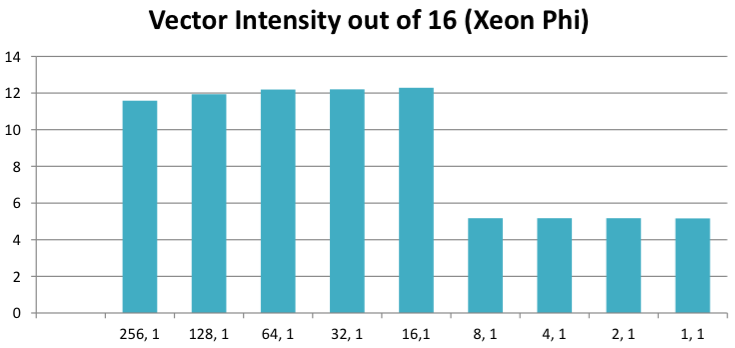
\includegraphics[width=0.8\textwidth]{figures/nbody_phi_vec.png}
    \caption{Vtune vector intensity Xeon Phi, Nbody.}
    \label{nbody_phi_vec}
\end{figure}

\par{Vtune results also showed that the values of 8 and 16 work items for 
    the CPU and Xeon Phi respectively had the lowest CPI rate. 
    \emph{``The CPI value of an application or function is an indication 
    of how much latency affected its execution. Higher CPI values mean 
    there was more latency in your system – on average, it took more 
    clockticks for an instruction to retire. Latency in your system 
    can be caused by cache misses, I/O, or other bottlenecks''}.\cite{cpi}}

\subsubsection{GPU}
\par{In Best case scenario, we have enough Work Groups to utilize all 
    Streaming Multiprocessors (SM), and also utilise all the cores 
    within due to enough local work items.}

{\centering{120 Work Groups > 13 Compute Units}\\}
{\centering{256 Work Items > 192 cores within each SM (compute unit)}\\}

\par{n the worst case scenario, we have enough Work Groups 
    to utilise all the SM's but the cores inside the SMs 
    are empty due to little amount of local work items. The results
    on the GPU are shown in figure \ref{nbody_gpu}.}

\begin{figure}[!h]
    \centering
    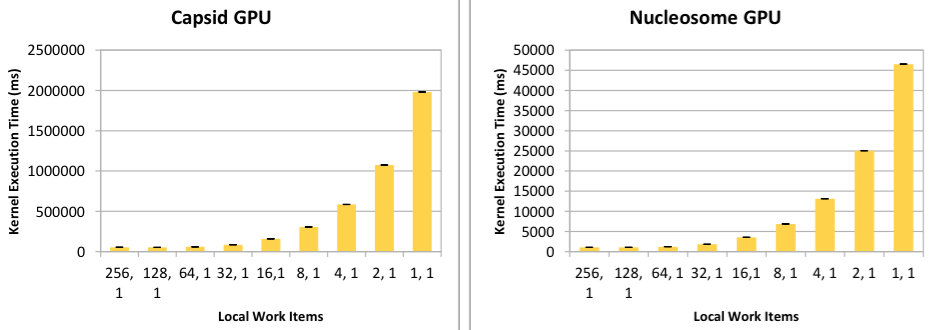
\includegraphics[width=0.8\textwidth]{figures/nbody_gpu.png}
    \caption{Graphical trends Nbody problem, Capsid and Nucleosome on GPU.}
    \label{nbody_gpu}
\end{figure}
        
\subsubsection{Comparision Xeon/Phi/GPU}
\par{Figure \ref{nbody_comp} shows that GPU emerges as the hardware with the 
    greatest performance. 
    This can be explained by the fact that the GPU has up to 64KB 
    Configurable Shared Memory and L1 Cache. Since the memory 
    access pattern of this kernel is coalesced (explained further on), 
    having sufficient first level cache is a key contributor to good 
    performance. The Tesla K20 also has a peak theoretical performance 
    of 3.52 Teraflops 
    , which is almost twice the rate for the Xeon Phi (~2 Tflops). 
    Also, due to the inherent level of parallelism in the kernel, 
    the GPU is a great fit with its greater length SIMD processors 
    and native support for parallelism with a large number of threads.}

\begin{figure}[!h]
    \centering
    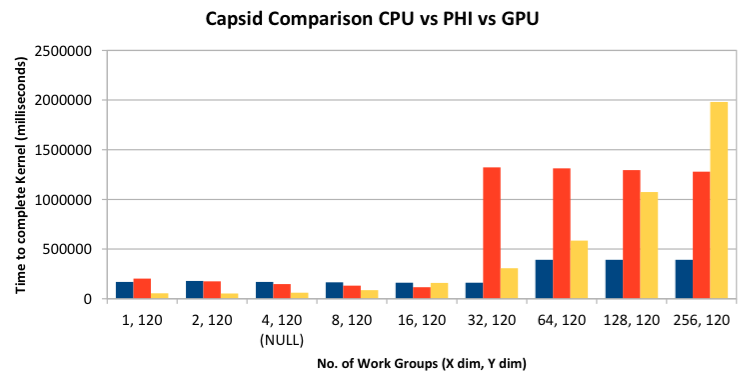
\includegraphics[width=0.8\textwidth]{figures/nbody_comp.png}
    \caption{Graphical trends Nbody problem, Capsid and Nucleosome comparison between architectures.}
    \label{nbody_comp}
\end{figure}

\par{As with the CPU and Xeon Phi, it is immediately apparent 
    that the Xeon Phi has a much greater degree of response to 
    the under utilisation of vector units. This is because the CPU 
    is a smarter hardware which has better support for serialized 
    code in terms of branch prediction and a more sophisticated memory 
    management system.}



%------------------------------------------------
\section{Future Work and Conclusions}
\par{We successfully ported DL\_POLY to Xeon Phi and showed that without an intensive effort into optimisation it is 
difficult to fully take advantage of the Xeon Phi co-processor. Moderate success can be claimed for the OpenMP implementation were
we showed that for intensive routines with the right type of parallelism in native mode we can be as fast as the host, 
\emph{eg.} Shake. MPI symmetric seems to be a no go area as long as the homogenous decomposition of data is maintained.
By far the most promising is the offload mode, where synchronous offloading showed encouraging results. Future work will 
concentrate on mixing asynchronous computation and data transfers as promising sources of speed-up.}

%------------------------------------------------
\phantomsection
\section*{Acknowledgments} % The \section*{} command stops section numbering
\addcontentsline{toc}{section}{Acknowledgments} % Adds this section to the table of contents with 
                                                % negative horizontal space equal to the indent for the numbered sections
\par{to be added}


%----------------------------------------------------------------------------------------
%	REFERENCE LIST
%----------------------------------------------------------------------------------------
\newpage
\phantomsection
%\nocite{*}
\bibliographystyle{unsrt}
\bibliography{report}

\phantomsection
\section*{Supplementary Information} % The \section*{} command stops section numbering
\addcontentsline{toc}{section}{Supplementary Information} % Adds this section to the table of contents with negative horizontal 
                                                        %space equal to the indent for the numbered sections
\par{...}

%----------------------------------------------------------------------------------------

\end{document}
